\tikzset{every picture/.style={line width=0.75pt}} %set default line width to 0.75pt        

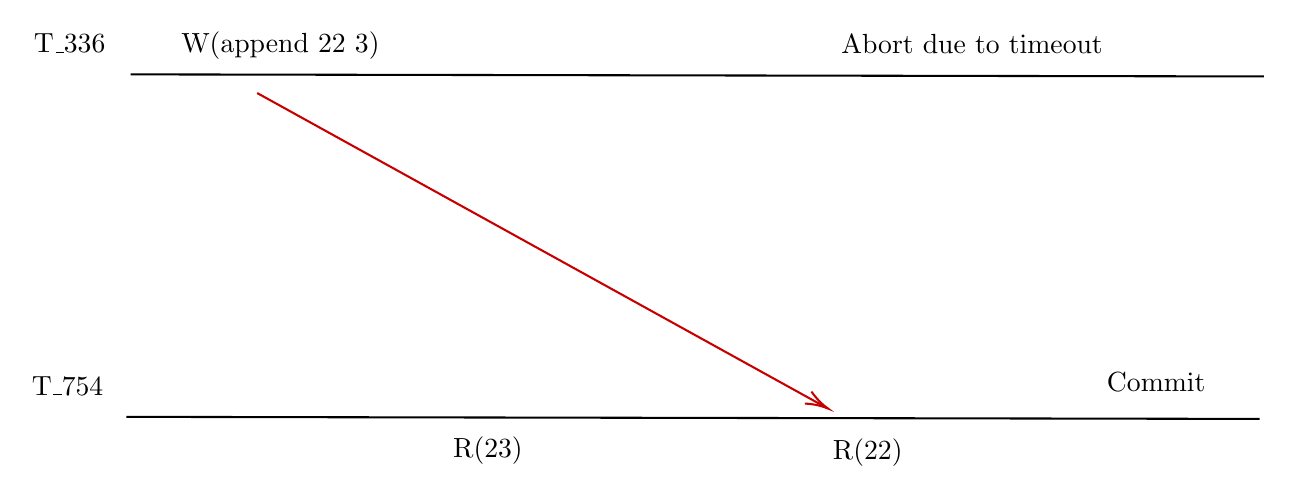
\begin{tikzpicture}[x=0.75pt,y=0.75pt,yscale=-1,xscale=1]
%uncomment if require: \path (0,300); %set diagram left start at 0, and has height of 300

%Straight Lines [id:da9500410641573396] 
\draw    (62.09,31) -- (608.09,32) ;
%Straight Lines [id:da7796185686481738] 
\draw    (60.09,196) -- (606.09,197) ;
%Straight Lines [id:da424831019884359] 
\draw [color={rgb, 255:red, 198; green, 0; blue, 0 }  ,draw opacity=1 ]   (123.09,40) -- (396.34,191.03) ;
\draw [shift={(398.09,192)}, rotate = 208.93] [color={rgb, 255:red, 198; green, 0; blue, 0 }  ,draw opacity=1 ][line width=0.75]    (10.93,-3.29) .. controls (6.95,-1.4) and (3.31,-0.3) .. (0,0) .. controls (3.31,0.3) and (6.95,1.4) .. (10.93,3.29)   ;

% Text Node
\draw (14,10) node [anchor=north west][inner sep=0.75pt]   [align=left] {T\_336};
% Text Node
\draw (13,175) node [anchor=north west][inner sep=0.75pt]   [align=left] {T\_754};
% Text Node
\draw (85,9) node [anchor=north west][inner sep=0.75pt]   [align=left] {W(append 22 3)};
% Text Node
\draw (216,204) node [anchor=north west][inner sep=0.75pt]   [align=left] {R(23)};
% Text Node
\draw (399,205) node [anchor=north west][inner sep=0.75pt]   [align=left] {R(22)};
% Text Node
\draw (403,10) node [anchor=north west][inner sep=0.75pt]   [align=left] {Abort due to timeout};
% Text Node
\draw (531,173) node [anchor=north west][inner sep=0.75pt]   [align=left] {Commit};
% Text Node
\draw (122,133) node [anchor=north west][inner sep=0.75pt]   [align=left] {};


\end{tikzpicture}


